\section{Word2Vec} \label{sec:Word2Vec}

\subsection{Word Embedding Representations: Count-Based vs. Context-Based} \label{sec:CountVsContextModels}
 
Word embeddings can be learned using two kinds of contextual vector space models: the \textbf{count-based} or \textbf{context-based vector space models}. 

\textbf{Count-based vector space models} are unsupervised learning algorithms based on matrix factorization of a global word co-occurrence matrix. The main assumption is words in similar contexts share related semantic meanings. Examples include PCA and neural probabilistic language models. Another term for this type is \textbf{distributed semantic model} (DSM) (Weng, 2017). 

\textbf{Context-based vector space models} are supervised algorithms that use a local context to predict target words. These are predictive models which take dense word vectors as parameters and update word representations during training.

In 2014, Baroni et al. showed that predictive approaches outperformed count models significantly and consistently. 

Although \textbf{Word2Vec} and \nameref{sec:Glove} are predictive and context-based vector space models, they still rely on co-occurrence counts. 

\textbf{Word2Vec} is an unsupervised learning algorithm for obtaining word vector representations using a two-layer neural network. Its input is the text corpus and output is the set of feature vectors, as one vector per word. Existing word representations already capture linguistic patterns, allowing algebraic operations to be done on the word vectors in their semantic vector space; for example, $vector(\textit{"King"}) - vector(\textit{"Man"}) + vector(\textit{"Woman"})$ outputs a vector close to the word vector for ``Queen". But Mikolov et al. (2013b) created the \nameref{sec:SkipGram} and \nameref{sec:CBOW} as part of \textbf{Word2Vec} to learn word vector representations more efficiently from large data. Previous architectures used fewer words and smaller vector dimensionality, thus reducing the quality of the learned representations. 

\subsubsection{One-Hot Encodings} \label{sec:OneHotEncodings}

A key concept for what follows is \textbf{one-hot vector encoding}. This is the simplest type of word embedding where each cell in the vector corresponds to a distinct vocabulary word, thus its dimension equals the vocabulary size. A $1$ is placed in the cell marking the position of the word in the vocabulary, and a $0$ is placed in all other cells. However, this can result in high-dimensionality vector representations for large vocabularies, causing increased computational costs, and similarity between categories cannot be represented. 

\subsection{Basic Structure of Skip-Gram and CBOW} \label{sec:BasicSkipGramAndCBOW}

Both the \nameref{sec:SkipGram} and \nameref{sec:CBOW} are \hyperref[sec:NeuralLM]{neural network language models} with one hidden layer.  

The input vector $\overrightarrow{x} = (x_1,..., x_V)$ and output vector $\overrightarrow{y} = (y_1,...,y_V)$ are both \textbf{\hyperref[sec:OneHotEncodings]{one-hot encodings}}, and the hidden layer of the \hyperref[sec:NeuralLM]{neural network} is a \hyperref[sec:WordEmbeddings]{word embedding} with dimension $N$. (Thus even though the vocabulary size is $V$, the goal is to learn embeddings with size $N$). For a specific time step $t$, the model predicts one output word $w_{t+j}$ whose vector representation is $\overrightarrow{y}$, given one input word $w_t$, whose vector representation is $\overrightarrow{x}$.   

For \textbf{Skip-Gram}, $w_{t+j}$ is the predicted context word and $w_t$ is the input target word, but for \textbf{CBOW} $w_{t+j}$ is the predicted target word and $w_t$ is the input context word.   

Vectors $v_w$ and $v'_w$ are two representations of word $w$. Vector $v_w$ comes from the rows of the \textit{input layer $\rightarrow$ hidden layer weight matrix} $W$, and vector $v'_w$ comes from the rows of the \textit{hidden layer $\rightarrow$ output layer weight matrix} $W'$. We call $v_w$ the \textbf{input vector} and $v'_w$ is the \textbf{output vector} of the word $w$. 


\subsubsection{Skip-Gram Model} \label{sec:SkipGram}

The Skip-Gram model predicts context words given a single target word. It uses a fixed sliding window $c$, or size of the training context, to capture context along a sentence. A target word thus has left and right context words within that sliding window. This target center word is represented as a one-hot encoding that is input to a neural network which updates the vector with values near $1$ in cells corresponding to predicted context words (Weng, 2017).  

Consider the following sentence from Weng (2017): ``The man who passes the sentence should swing the sword." Using a context window size of $c = 5$ and target word ``swing", the Skip-Gram should learn to predict the context words $\{\texttt{"sentence"}, \texttt{"should"}, \texttt{"the"}, \texttt{"sword"} \}$, and so the target-context word pairs fed into the model for training are: (\texttt{"swing"}, \texttt{"sentence"}), (\texttt{"swing"}, \texttt{"should"}), (\texttt{"swing"}, \texttt{"the"}), and (\texttt{"swing"}, \texttt{"sword"}).  

\begin{figure}[h]
\vspace{-5pt}
\centering
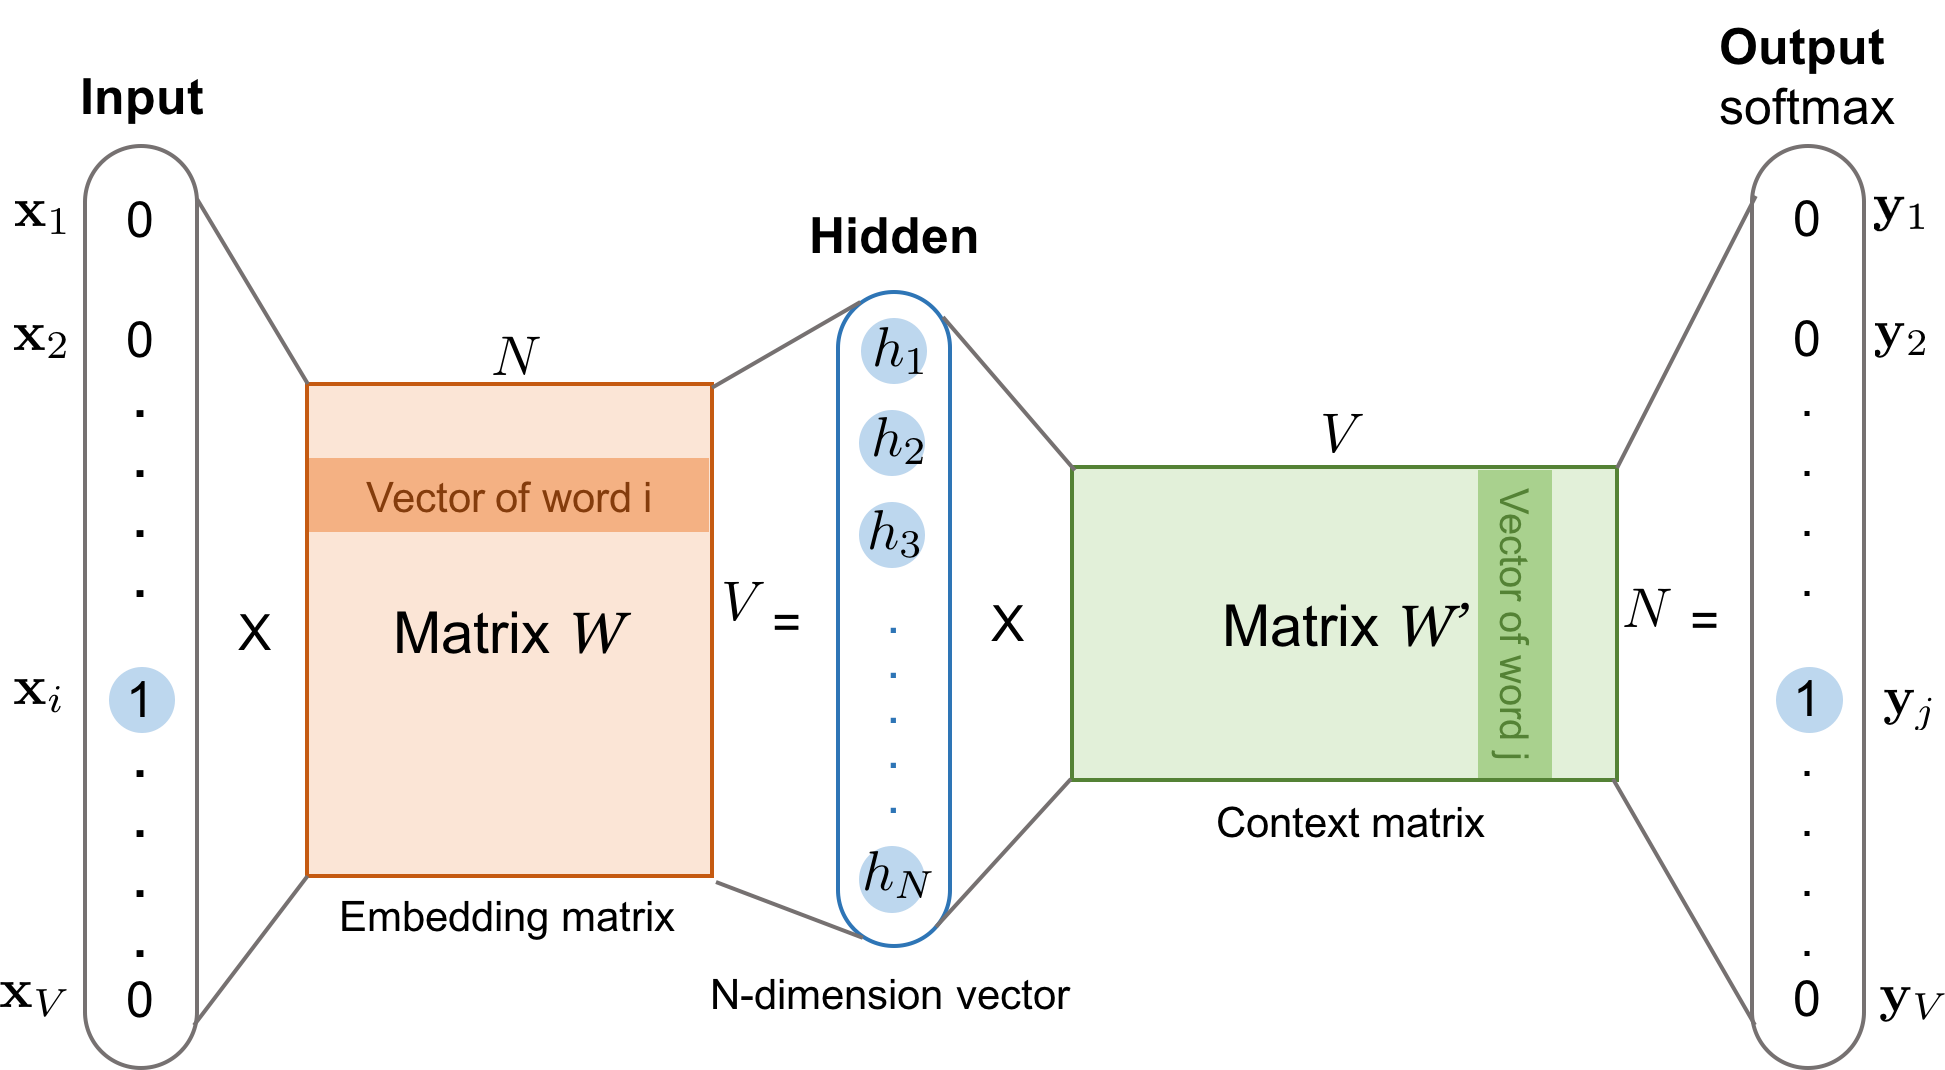
\includegraphics[width=0.6\textwidth]{imgs/skipgram_image.png}
\vspace{-5pt}
\caption{\footnotesize Skip-Gram Model; simplified version, with one input target word and one output context word. From \emph{Learning Word Embeddings}, by Lilian Weng, 2017. \url{https://lilianweng.github.io/lil-log/2017/10/15/learning-word-embedding.html}. Copyright n.d. by n.d.}
\label{fig:SkipGram}
\vspace{-5pt}
\end{figure}

\subsubsection{Forward and Backward Pass for Skip-Gram}

According to the Skip-Gram illustrated in \cref{fig:SkipGram}, the procedure for learning word vectors is: 
\begin{enumerate}
    \item the input word $w_i$ and output word $w_j$ are encoded as one-hot vectors, $\overrightarrow{x}$ and $\overrightarrow{y}$ respectively. (For Skip-Gram, $\overrightarrow{x}$ is the target vector and $\overrightarrow{y}$ is the context vector). 
    
    \item A randomly initialized word embedding matrix $W$ with size $V \times N$ at the input $\rightarrow$ hidden layer is multiplied with $\overrightarrow{x}$ to give the $N$-dimensional embedding for target word $w_i$. This embedding resides in the $i$-th row of $W$ and is considered as the hidden layer of the model. 
    
    \item Next, the hidden layer is multiplied by weight matrix $W'$ with size $N \times V$ to produce the one-hot encoded output vector, $\overrightarrow{y}$. \textbf{NOTE: }the output context matrix $W'$ encodes words as context and is distinct from the embedding matrix $W$. 
    
    \item The result of the above multiplication is sent through the softmax layer to create a probability distribution over the words. The above steps constitute the \hyperref[sec:ForwardProp]{forward pass}.
    
    \item \hyperref[sec:ErrorCalc]{Errors} are obtained by subtracting the output vector with the target vector. 
    
    \item The error vector is \hyperref[sec:BackwardProp]{backward-propagated} through the neural network to update the weight matrix. The procedure continues until errors are small enough. 
    
\end{enumerate}


\subsubsection{Loss Function for Skip-Gram}

The loss function is a key step for backward propagating errors through the neural network. Mikolov et al. (2013a) defines the loss function to be able to find word representations to predict the output word $w_{t+j}$ given an input word $w_t$. Formally, given the training word sequence $w_1, w_2, ..., w_T$ with $T$ training samples, the Skip-Gram maximizes the average log probability
$$
J_\theta = \frac{1}{T} \sum_{t=1}^T \sum_{-c \leq j \leq c, j \neq 0} \text{log} \Big(P \Big(w_{t+j} \;| \; w_t \Big) \Big)
$$
where $c$ is the training size context window. 

From Peters et al. (2013), the above probability in the loss function is:
$$
P \Big( w_{t+j} \; | \; w_t \Big) = \frac {\exp{ \Big( (v'_{w_{t+j}})^T  v_{w_t} \Big) }} {\sum_{w=1}^V \exp{ \Big( (v'_w)^T \cdot v_{w_t} \Big) }}
$$
where $w_t$ is the inputted target word, $w_{t+j}$ is the predicted context word, and $V$ is the number of vocabulary words. 
 

%\nameref{app:Appendix_SkipGram} applies the Skip-Gram model to neural translation, using the word embedding concept. 


\subsubsection{Continuous Bag of Words Model (CBOW)} \label{sec:CBOW}

The continuous bag of words model (CBOW) is opposite of the Skip-Gram since it predicts the \emph{target} word based on a \emph{context} word. In the general case, CBOW receives a window of $n$ context words around the target word $w_t$ at each time step $t$ and tries to predict the target word. The CBOW in \cref{fig:CBOW} is called ``continuous" bag-of-words since it uses continuous distributed representations of the context words whose order is not important (Mikolov et al., 2013b). 

\begin{figure}[h] 
\vspace{-5pt}
\centering
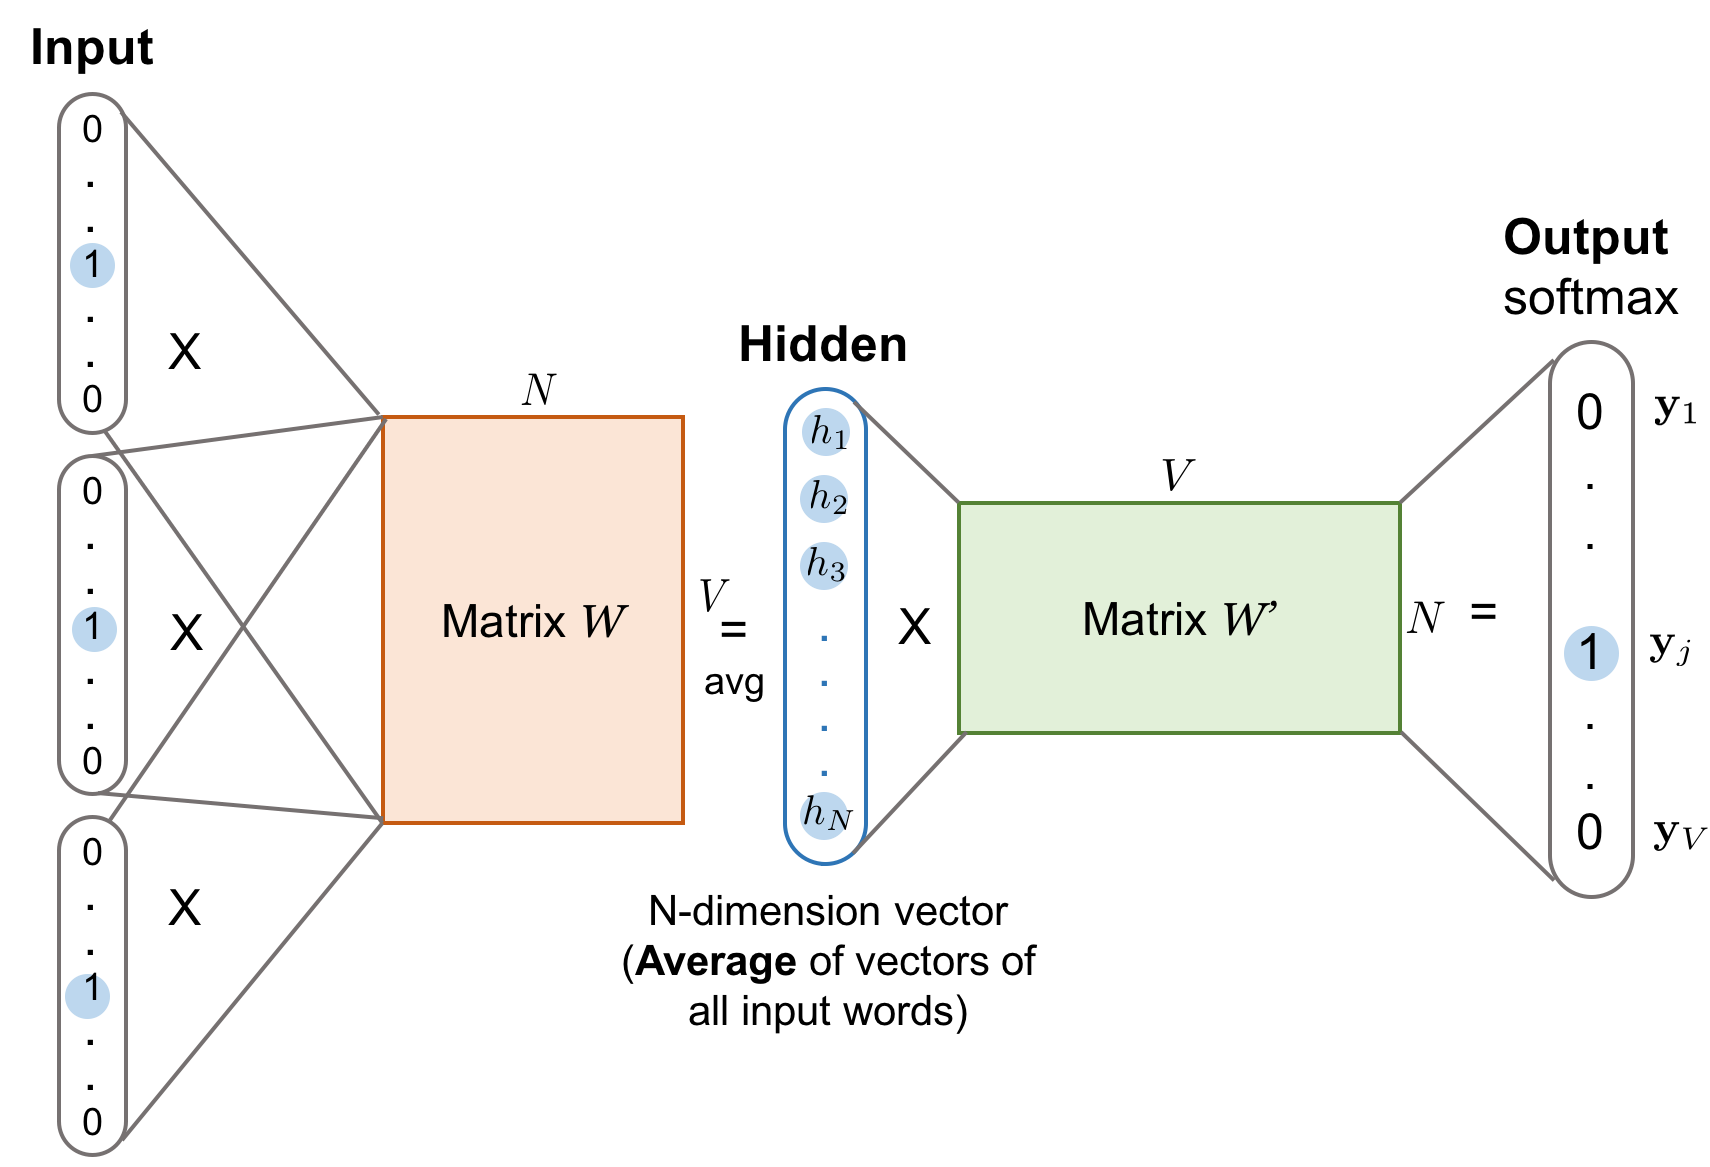
\includegraphics[width=0.6\textwidth]{imgs/cbow.png}
\vspace{-5pt}
\caption{\footnotesize CBOW Model with several one-hot encoded context words at the input layer and one target word at the output layer. From \emph{Learning Word Embeddings}, by Lilian Weng, 2017. \url{https://lilianweng.github.io/lil-log/2017/10/15/learning-word-embedding.html}. Copyright n.d. by n.d.}
\label{fig:CBOW}
\vspace{-5pt}
\end{figure}

\subsubsection{Forward and Backward Pass for CBOW}

The forward pass for CBOW is similar to Skip-Gram's. The key difference is due to having multiple context words: the CBOW averages the context word vectors while multiplying the input vector $\overrightarrow{x}$ and input $\rightarrow$ hidden layer matrix $W$. Rong (2016) describes the hidden layer calculation as: 
$$
\begin{array}{ll}
\overrightarrow{h} 
&= \frac{1}{c} W \cdot \Big(\overrightarrow{x_1} + \overrightarrow{x_2} + ... + \overrightarrow{x_c} \Big) \\
&= \frac{1}{c} \cdot \Big(\overrightarrow{v_{w_1}} + \overrightarrow{v_{w_2}} + ... + \overrightarrow{v_{w_c}} \Big)
\end{array}
$$
where $c$ is the number of context words, $w_1,...,w_c$ are the context words, and $v_w$ is the input vector for general word $w$. According to Weng (2016), the fact that CBOW averages distributional information of the context vectors makes it better suited for small datasets. 

\subsubsection{Loss Function for CBOW}

On the output layer, the CBOW outputs $c$ multinomial distributions, for each of the $c$ context words. The training object is to maximize the conditional probability of observing the true output word given several context words, while accounting for their weights. 

From Ruder (2016), the loss function is: 
$$
J_\theta = \frac{1}{T} \sum_{t=1}^T \text{log} \Big( P \Big( w_t \; | \; w_{t-n}, ..., w_{t-1}, w_{t+1}, ..., w_{t+n} \Big) \Big)
$$
where $n$ is number of context words and $w_{t-n}, ..., w_{t+n}$ are context words around the target word $w_t$. 

From Rong (2016), the above probability in the loss function, for the one context word case, is:
$$
P \Big( w_t \; | \; w_I \Big) = \frac {\exp{ \Big( (v'_{w_O})^T  v_{w_I} \Big) }} {\sum_{w=1}^V \exp{ \Big( (v'_w)^T \cdot v_{w_I} \Big) }}
$$
where $w_I$ is the input context word, $w_O$ is the predicted target word, and $V$ is the number of vocabulary words. 
  
%\nameref{app:Appendix_CBOW} applies the CBOW model to \nameref{nlptask:machinetranslationMT}, using the \hyperref[sec:WordEmbeddings]{word embedding} concept. 


\subsection{Phrase-Learning in Word2Vec Using Skip-Gram}

Mikolov et al. (2013a) state that a problem with previous word vectors is their lack of phrase representation - the phrases ``Canada" and ``Air" could not be recognized as part of a larger concept and thus combined into ``Air Canada". Many phrases have meaning that is not just a composition of the meanings of its individual words and should be represented as their own unique tokens in the training data. In contrast, a bigram like ``this is" should remain unchanged (Mikolov et al., 2013a, p. 5). 

To solve this issue, the Skip-Gram was updated using a data-driven scoring technique. Phrases are formed based on unigram and bigram counts: 
$$
S_{phrase} = \frac{C(w_i w_j) - \delta} {C(w_i)C(w_j)}
$$
where $C(\cdot)$ is the count of a unigram $w_i$ or bigram $w_i w_j$ and $\delta$ is a discounting threshold to avoid formation of infrequent words and phrases. High values of $S_{phrase}$ means the phrase is most likely a phrase rather the simple concatenation of two words. 

Regarding model accuracy, Mikolov et al. (2013a) found that the phrase Skip-Gram model with hierarchical softmax and subsampling performed significantly better on a large data set than the original Skip-Gram without the phrase feature. 

It was found that the phrase Skip-Gram exhibits a linear structure \textbf{additive compositionality} of word vectors, which allows words to be combined meaningfully by adding their word vectors. For instance, composing word vectors $vector(\texttt{"French"}) \! + \! vector(\texttt{"actress"})$ results in the phrase $vector(\texttt{"Juliette Binoche"})$. 

This \textbf{additive compositionality} feature of word vectors stems from the loss function's formulation. Since learned context vectors can represent the overall distribution of context words in which the target word appears, and since the vectors are logarithmically related to the probabilities from the output layer, the sum of two word vectors is related to the product of the context distributions (using the logarithm sum rule). This product of distributions functions like an AND function since words are weighted by probability. Consequently, if the key phrase ``Volga River" appears many times in the same sentence along with ``Russian" and ``river", the sum $vector(\texttt{"Russian"}) \! + \! vector(\texttt{"river"})$ results in the phrase $vector(\texttt{"Volga River"})$ or at least a vector close to it (Mikolov et al., 2013a). 
